\documentclass{article}
\usepackage[spanish]{babel}
\usepackage[numbers,sort&compress]{natbib}
\usepackage{graphicx}

\graphicspath{ {images/} }
\usepackage{subfigure}
\usepackage{url}
\usepackage{hyperref}
\usepackage{amsmath}
\usepackage[top=15mm, bottom=40mm, left=15mm, right=15mm]{geometry}
\setlength{\parskip}{2mm}
\setlength{\parindent}{0pt}
\usepackage{listings}
\usepackage{mathrsfs}


\lstdefinestyle{mystyle}{
  numbers= left}
\lstset{style=mystyle}

\author{3175}
\title{Práctica 9: Interacciones entre partículas}
\date{\today}

\begin{document}

\maketitle


\section{Introducción}

Las fuerzas entre partículas son muchas y variadas, entre las mas importantes están las fuerzas electroestáticas proporcionadas por las cargas que éstas poseen la cual determina si se atraen o se repelen y la fuerza de gravedad que afecta a todo aquello que tiene una masa o inclusive una masa aparente como lo es en el caso de algunas partículas como los electrones.\citep{web1}.
 
\section{Objetivo}
En base a un modelo de interacción entre elementos determinado por una simulación simple de cargas, agregar un factor adicional de un fenómeno como es la gravedad también de manera simple para comparar como éstos dos fenómenos influyen en el comportamiento de los elementos dentro del sistema tomando como referencia la velocidad de éstos.

\section{Metodología}

Usando de base el código proporcionado\citep{webelisa}, se definen cincuenta elementos a los que consideramos partículas $n$ cada una con una posición $x$ y $y$, carga $c$ [figura 1] y posteriormente se agrega un valor de masa $m$ definido en base a valores dentro de una distribución normal en valores positivos de cero a uno, con excepción de las cargas donde éstos valores pueden ser negativos entre menos uno y uno, el signo del valor de la carga describe su carga, la cual es necesaria para determinar si se atraen o se repelen dos partículas.

Dentro de la función de fuerza se deben incluir los criterios que definen el comportamiento por derivado de la masa, el cual es la fuerza de gravedad tomando en cuenta cual partícula tiene mas masa que es la que va a atraer a la otra definiendo la dirección del movimiento de la fuerza, para finalmente aplicarse a las fuerzas totales que inciden. Se realiza ésto para las fuerzas totales, para solo las cárgas (como en el código base) y solamente tomando en cuenta la masa.

\lstinputlisting[language= R, firstline=43, lastline=43]{P9.R}
\lstinputlisting[language= R, firstline=47, lastline=47]{P9.R}
\lstinputlisting[language= R, firstline=50, lastline=43]{P9.R}

Finalmente se realizan las iteraciones para las cincuenta partículas en un lapso de tiempo de cien pasos tomando en cuenta los tres criterios antes mencionados. Definendo los cambios $delta$ de posición diferentes para cada caso, en cada paso que es la unidad de tiempo.

\lstinputlisting[language= R, firstline=111, lastline=126]{P9.R}


\section{Resultados}
Los resultados en la figura 2 muestran el comportamiento del sistema de partículas representado por líneas que describen el comportamiento de la velocidad, en el cual se aprecia la velocidad con cargas en color azul, la velocidad con masas en color negro y la combinación de ambas en línea amarilla.


\section{Conclusiones}
Se puede determinar en base a la gráfica que el comportamiento de la velocidad de las partículas con ambos fenómenos se ve mas fuertemente influenciado por la fuerza de gravedad que por las cargas, que sin embargo, si modifica visiblemente el comportamiento de la velocidad pero en menor medida
\begin{figure}[h]
\centering
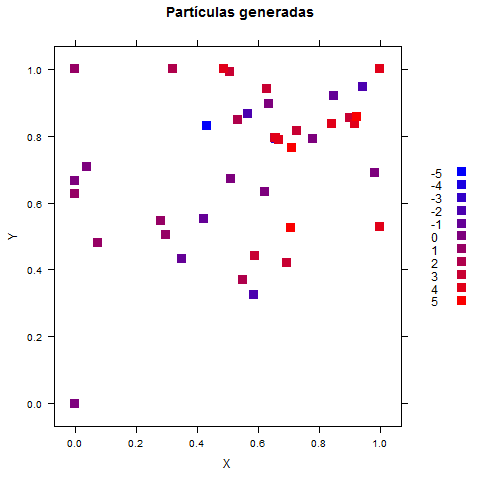
\includegraphics[width=7cm, height=7cm]{p9i.png}
\caption{Posiciones iniciales de las partículas}
\end{figure}

\begin{figure}[!ht]
\centering
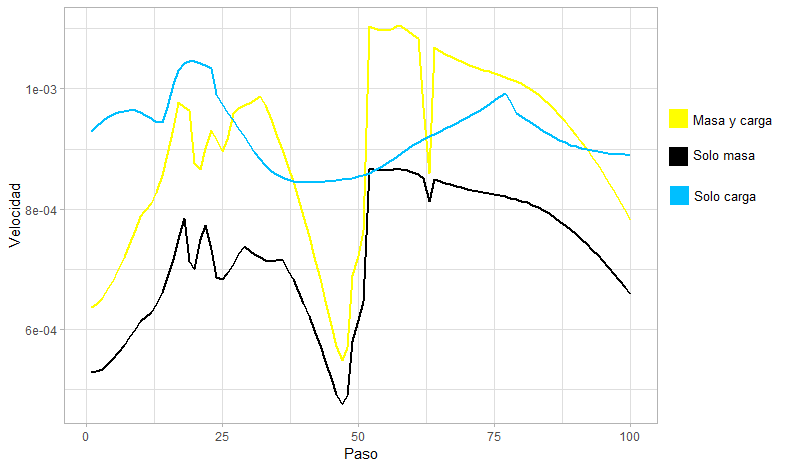
\includegraphics[width=12cm]{Grafica.png}
\caption{Gráfica de velocidades}
\end{figure}



\bibliographystyle{plainnat}
\bibliography{bibP9}
\end{document}